\documentclass[11pt,english,french]{scrreprt}
\usepackage{lmodern}
\usepackage{babel}
\renewcommand{\familydefault}{\rmdefault}
\usepackage[T1]{fontenc}
\usepackage{ucs}
\usepackage[utf8x]{inputenc}
\usepackage[a4paper]{geometry}
\geometry{verbose,tmargin=2cm,bmargin=2cm,lmargin=2cm,rmargin=2cm,headheight=2cm,footskip=1cm}
\setlength{\parskip}{\smallskipamount}
\setlength{\parindent}{0pt}

\usepackage{amsthm}
\usepackage{booktabs}
\usepackage{amsmath}
\usepackage[unicode=true, pdfusetitle,
 bookmarks=true,bookmarksnumbered=false,bookmarksopen=false,
 breaklinks=false,pdfborder={0 0 1},backref=false,colorlinks=false]
 {hyperref}

\makeatletter
\usepackage{colortbl}
\usepackage{color}
\usepackage[dvipsnames]{xcolor}
\usepackage{wrapfig}
\usepackage{graphicx}
\usepackage{listings}
\usepackage[calcwidth]{titlesec}
\usepackage{fix-cm}
\usepackage{multicol}
\usepackage{verbatim}
\usepackage{moreverb}
\usepackage{nicefrac}
\usepackage{amssymb}
\usepackage{array}
\usepackage{tabularx}
\usepackage{subfig}
\usepackage[french,ruled,vlined]{algorithm2e}
\SetAlgoProcName{Procédure}{proc}

\theoremstyle{remark}
  \newtheorem*{rem*}{Remarque}
\theoremstyle{definition}
  \newtheorem*{defi}{Définition}
  \newtheorem{ques}{Question}[section]

\definecolor{MyDarkBlue}{rgb}{0,0.08,0.45}

\definecolor{pink}  {rgb}{0.67, 0.05, 0.57} % keywords
\definecolor{red}   {rgb}{0.87, 0.20, 0.00} % strings
\definecolor{green} {rgb}{0.00, 0.47, 0.00} % comments
\definecolor{violet}{rgb}{0.41, 0.12, 0.61} % classes
\definecolor{blue}  {rgb}{0.21, 0.00, 0.44} % functions
\definecolor{brown} {rgb}{0.39, 0.22, 0.13} % brown

\lstdefinestyle{Xcode} {
    language        = C,
    basicstyle      = \small\ttfamily,
    identifierstyle = \textcolor{black},
    commentstyle    = \textcolor{green},
    keywordstyle    = \textcolor{pink},
    stringstyle     = \textcolor{red},
    directivestyle  = \textcolor{brown},
    extendedchars   = true,
    tabsize         = 4,
    showspaces      = false,
    showstringspaces = false,
    breakautoindent = true,
    flexiblecolumns = true,
    keepspaces      = true,
    stepnumber      = 0,
    xleftmargin     = 0pt}

\lstset{style=Xcode}

\titleformat{\section}[hang]{\sffamily\bfseries}
 {\Large\thesection}{12pt}{\Large}[{\titlerule[0.5pt]}]

\def\thickhrulefill{\leavevmode \leaders \hrule height 1pt\hfill \kern \z@}
\renewcommand{\maketitle}{\begingroup%
    \let\footnotesize\small
    \let\footnoterule\relax
    \parindent \z@
    \reset@font
    \begin{flushleft}
      \huge \sffamily \bfseries\color{orange} \@title
    \end{flushleft}
    \hrule height 1pt
    \begin{flushright}
      \large\sffamily\color{MyDarkBlue}\@author
    \end{flushright}
  \endgroup%
  \setcounter{footnote}{0}%
}

\AtBeginDocument{
  \def\labelitemi{\normalfont\bfseries{--}}
}

\makeatletter
\renewcommand\thesection{\arabic{section}}
\@addtoreset{section}{chapter}
\makeatother

\makeatother
\begin{document}
	
\title{LI312 - Examen 2008}
\author{Benjamin BARON}

\maketitle

\section{Caches} % (fold)

Soit un processeur MIPS associé à un cache de données à correspondance directe. Ce cache possède une capacité totale de stockage de 1 Ko ($=1\,024$ octets). On rappelle que toutes les adresses émises par le processeur sont des adresses octets, et les adresses sont codées sur 32 bits. On ne s'intéresse dans cet exercice qu'au cache de données, et chaque ligne du cache de données possède une longueur de 64 octets.

On considère une matrice carrée A de $16\times 16$ entiers : pour tout couple d'entiers $(i,\,j),\;0\leqslant i,\,j\leqslant 15$,  $A[i,\,j]$ désigne l'entier de la ligne $i$ et la colonne $j$. La matrice est stockée en mémoire à l'adresse $A=\texttt{0x00000 17C00}$. Chaque entier est représenté par un mot de 32 bits, l'entier $A[i,\,j]$ est ainsi stocké à l'adresse $A+(16\times i+j)\times4$.

\begin{figure}[h]
	\center
	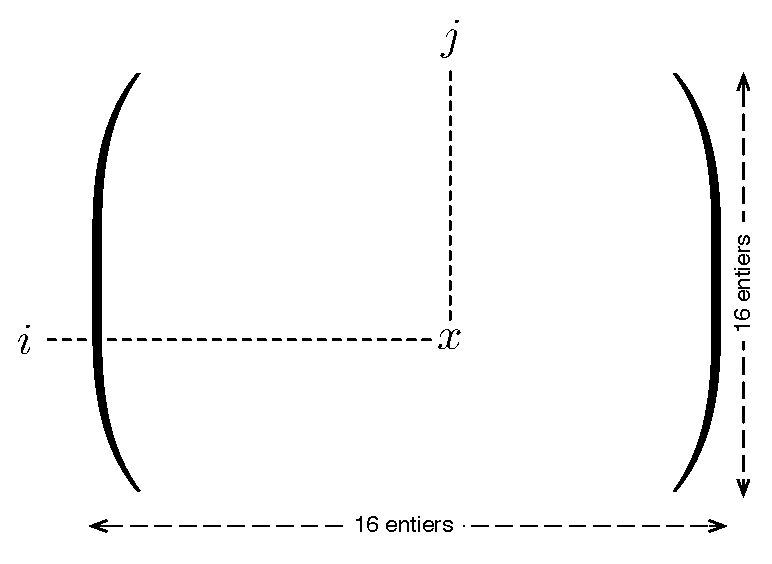
\includegraphics[scale=.5]{diagrammes/matrice}
\end{figure}

\begin{ques}
	On rappelle qu'une case du cache est un emplacement pouvant contenir une ligne de cache complète.
	
	Nombre $NbC$ de cases du cache : $NbC = \nicefrac{1024}{64}=\nicefrac{2^{10}}{2^6}=2^4=16$.
	
	Une ligne de cache complète peut alors contenir $\nicefrac{64}{4} = 16$ mots de 32 bits.
	
	Le nombre de bits de l'\emph{index} est donc égal à $\log_2(16) = 4$. L'index désigne une case dans le cache.
	
	Le nombre de bits de l'\emph{offset} est égal à $\log_2(64) = 6$. L'offset désigne un octet dans une case du cache.
	
	\begin{figure}[h]
		\center
		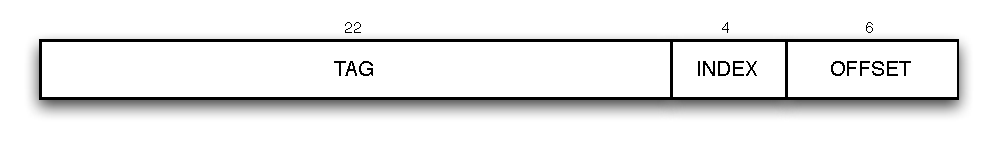
\includegraphics[scale=.9]{diagrammes/part-adresse}
	\end{figure}
\end{ques}

\begin{ques}
	La matrice $A$  s'étend de l'adresse
	\[\texttt{0001 0111 1100 0000 0000}\;(\texttt{0x1 7C00})\]
	à l'adresse
	\[\texttt{0001 0111 1111 1111 1100}\;(\texttt{0x1 7FFC})\]
	
	La seule adresse pouvant occuper le mot 0 ($\textrm{offset} = 0$) de la ligne 0 ($\textrm{index} = 0$) du cache est alors le mot $A[0,\,0]$ placé à l'adresse \texttt{0x0001 7C00}.
	
	D'une manière générale, les éléments $A[c,\,k]$ de la matrice $A$ occuperont le mot $k$ ($\mathrm{offset} = k$) de la case $c$ ($\mathrm{index} = c$) du cache.
\end{ques}

\begin{ques}

	On souhaite exécuter le code suivant (on suppose la variable $S$ initialisée au préalable) : 
\begin{lstlisting}
for(j = 0; j < N; j++) {
	for(i = 0; i < N; i++) {
		S += A[i,j];
	}
}
\end{lstlisting}

	Remplir le tableau ci-après pour la valeur $N=3$ en indiquant pour les 9 sommes effectuées, la valeur du couple $(i,\,j)$ et si l'accès au cache de données pour lire l'entier $A[i,\,j]$ est un succès ou un échec.

	\begin{tabularx}{\textwidth}{llX}
		\toprule
		Somme & Valeur de $(i,\,j)$ & Succès / échec\tabularnewline
		\midrule
		\midrule
		1 & $(0,\,0)$ & Echec (remplissage de la ligne $(0,\,0)\dots (0,\,15)$)\tabularnewline
		\midrule
		2 & $(1,\,0)$ & Echec (remplissage de la ligne $(1,\,0)\dots (1,\,15)$)\tabularnewline
		\midrule
		3 & $(2,\,0)$ & Echec (remplissage de la ligne $(2,\,0)\dots (2,\,15)$)\tabularnewline
		\midrule
		4 & $(0,\,1)$ & Succès\tabularnewline
		\midrule
		5 & $(1,\,1)$ & Succès\tabularnewline
		\midrule
		6 & $(2,\,1)$ & Succès\tabularnewline
		\midrule
		7 & $(0,\,2)$ & Succès\tabularnewline
		\midrule
		8 & $(1,\,2)$ & Succès\tabularnewline
		\midrule
		9 & $(2,\,2)$ & Succès\tabularnewline
		\bottomrule
	\end{tabularx}

	Taux de MISS obtenu : $\nicefrac{3}{9} = \nicefrac{1}{3}$.
\end{ques}

\begin{ques}
	On considère maintenant le code suivant équivalent au précédent mais en permutant $i$ et $j$ : 
\begin{lstlisting}
for(i = 0; i < N; i++) {
	for(j = 0; j < N; j++)
		S += A[i,j];
	}
\end{lstlisting}
	
	Remplir le tableau suivant pour la valeur $N=3$ en indiquant pour les 9 sommes effectuées, la valeur du couple $(i,\,j)$ et si les accès au cache de données sont un succès ou un échec.
	
	\begin{tabularx}{\textwidth}{llX}
		\toprule
		Somme & Valeur de $(i,\,j)$ & Succès / échec\tabularnewline
		\midrule
		\midrule
		1 & $(0,\,0)$ & Echec (remplissage de la ligne $(0,\,0)\dots (0,\,15)$)\tabularnewline
		\midrule
		2 & $(0,\,1)$ & Succès\tabularnewline
		\midrule
		3 & $(0,\,2)$ & Succès\tabularnewline
		\midrule
		4 & $(1,\,0)$ & Echec (remplissage de la ligne $(1,\,0)\dots (1,\,15)$)\tabularnewline
		\midrule
		5 & $(1,\,1)$ & Succès\tabularnewline
		\midrule
		6 & $(1,\,2)$ & Succès\tabularnewline
		\midrule
		7 & $(2,\,0)$ & Echec (remplissage de la ligne $(2,\,0)\dots (2,\,15)$)\tabularnewline
		\midrule
		8 & $(2,\,1)$ & Succès\tabularnewline
		\midrule
		9 & $(2,\,2)$ & Succès\tabularnewline
		\bottomrule
	\end{tabularx}

	Taux de MISS obtenu : $\nicefrac{3}{9} = \nicefrac{1}{3}$.
\end{ques}

\clearpage

\section{Programmation assembleur} % (fold)

On désire manipuler une liste chaînée en mémoire dans la zone des variables globales initialisées. Chaque élément de cette liste est une structure contenant deux mots de 32 bits : un pointeur sur l'élément suivant (adresse sur 32 bits) et une valeur (entier sur 32 bits). 

En C, on aurait :
\begin{lstlisting}
struct liste {
	struct liste *NEXT;
	unisigned int VAL;
};
\end{lstlisting}

\begin{ques}
	Donner les directives d'assemblage permettant de réserver et d'initialiser dans le segment \lstinline!.data! les 4 éléments de liste qui auront respectivement pour adresses : \lstinline!elm1!, \lstinline!elm2!, \lstinline!elm3!, \lstinline!elm4!, et pour valeurs : 23, 44, 52, 2.
	
\begin{lstlisting}
.data
elm1: .word elm2, 23
elm2: .word elm3, 44
elm3: .word elm4, 52
elm4: .word 0, 2
\end{lstlisting}
\end{ques}

\begin{ques}
	Convention d'utilisation de la pile.
	
	Les trois fonctions de la pile sont : \begin{itemize}
		\item Transmission des arguments de la fonction appelante vers la fonction appelée ;
		\item Sauvegarde de la valeur des ``registres persistants'' ;
		\item Zone de travail : variables locales.
	\end{itemize}
	
	Il faut déplacer le pointeur de la pile dans le prologue d'une fonction :
\vspace{-5pt}
\begin{lstlisting}[escapechar=\%]
addiu $29, $29, %$-4\times (nv+nr+\max(na_i))$%
\end{lstlisting}
\vspace{-10pt}
où :\begin{itemize}
	\item $na = \max(na_i, 4)$ où $na_i$ représente ne nombre d’arguments des fonctions $g_i$ appelées par $f$ ;
	\item $nv$ est le nombre de variables locales utilisées en C ;
	\item $nr$ est le nombre de registres persistants utilisés + \$31.
\end{itemize}

La fonction renvoie la valeur de retour est conventionnellement écrite dans le registre \$2 par la fonction appelée.
\end{ques}

\begin{ques}
	On veut écrire une fonction qui parcourt la liste et retourne la plus grande valeur de la liste. Cette fonction prend comme argument un pointeur sur le premier élément de la liste. 
	
	Le code C de la fonction est le suivant :
\begin{lstlisting}
void pg(struct liste *pl) {
	unsigned int max = 0;
	while (pl != NULL) {
		if (pl->VAL > max) 
			max = pl->VAL; 
		pl = pl->NEXT;
	} 
	return max;
}
\end{lstlisting}

	On rappelle que la notation \lstinline!pl->VAL! a la signification suivante : si \lstinline!pl! est l'adresse de base de la structure, \lstinline!pl->VAL! est la valeur dans le champ \lstinline!VAL! de la structure.
	
	Écrire cette fonction en assembleur MIPS R3000, en respectant les conventions d'utilisation de la pile. La variable locale \lstinline!max! sera implantée dans un registre, et il n'est donc pas nécessaire de réserver de la place dans la pile pour cette variable. On écrira cette fonction en utilisant les registres suivants :\begin{itemize}
		\item \$9 : adresse de la structure ;
		\item \$10 : champ \lstinline!VAL! de la structure ;
		\item \$11 : registre de travail ;
		\item \$2 : valeur de \lstinline!max! (à retourner par la fonction)
	\end{itemize}	 	
\begin{verbatimtab}[4]
pg:
#prologue
	addiu	$29,	$29,	-4		# seulement $31
	sw		$31,	0($29)

#corps
	xor		$2,		$2,		$2 		# max = 0
	or		$9,		$4,		$0		# $9 = @structure

boucle:
	beq		$9, 	$0, 	fin		# Si pl == NULL, fin de la fonction
	lw 		$10, 	4($9)			# $10 = pl->VAL
	slt 	$11, 	$2, 	$10		# Si max < pl->VAL alors $11 = 1
	beq 	$11, 	$0, 	faux
	or 		$2, 	$10, 	$0		# $ max = pl->VAL

faux:
	lw 		$9, 	0($9)			# pl = pl->NEXT
	j 		boucle

fin:

#epilogue
	lw 		$31, 	0($29)
	addiu 	$29, 	$29, 	4
	jr 		$31
\end{verbatimtab}
\end{ques}

\begin{ques}
	Ecrire le programme \lstinline!main()! qui appelle la fonction \lstinline!pg()!, et imprime le résultat sur le terminal au moyen d'un appel système.
\begin{verbatimtab}[4]
.text
	.globl main
#prologue
	addiu 	$29, 	$29, 	-8 		# $31 + 1 passage d'argument a la fonction pg
	sw 		$31, 	4($29) 			# sauvegarde de $31

# Corps
	la		$4, 	elm1			# $4 = @elm1
	jal		pg
# printf
	or 		$4, 	$2, 	$0
	ori 	$2, 	$0, 	1
	syscall

# Fonction terminale : inutile de retablir la pile
# exit
	ori 	$2, 	$0, 	10
	syscall
\end{verbatimtab}
\end{ques}

\end{document}